% =============================================================================
% FacebookEyeTracker — arXiv-style technical report
% Compile: pdflatex main.tex && bibtex main && pdflatex main.tex && pdflatex main.tex
% =============================================================================
\documentclass[11pt,a4paper]{article}

% ---------- packages ---------------------------------------------------------
\usepackage[utf8]{inputenc}
\usepackage[T1]{fontenc}
\usepackage{amsmath,amssymb}
\usepackage{graphicx}
\usepackage[hidelinks]{hyperref}
\usepackage{booktabs}
\usepackage{xcolor}
\usepackage[margin=2.5cm]{geometry}
\usepackage{tikz}
\usetikzlibrary{shapes.geometric, arrows.meta, positioning, calc}
\usepackage{caption}
\usepackage{subcaption}
\usepackage{natbib}
\usepackage{url}

% ---------- metadata ---------------------------------------------------------
\title{%
  FacebookEyeTracker: An Open-Source Pipeline for Collecting, Processing,
  and Visualizing Eye-Tracking Data on Social Media Content%
}

\author{
  Sebastian Breguel \\
  Pontificia Universidad Cat\'olica de Chile \\
  \texttt{sebabreguel@uc.cl}
}

\date{\today}

% =============================================================================
\begin{document}
\maketitle

% ---------- abstract ---------------------------------------------------------
\begin{abstract}
We present \textbf{FacebookEyeTracker}, an open-source pipeline for
collecting, processing, and visualizing eye-tracking data while users
browse social media feeds. The system captures binocular gaze data via
Tobii Pro hardware at ${\sim}60$\,Hz, cleans and interpolates tracking
gaps, temporally aligns gaze samples with individual posts, and generates
Gaussian heatmaps and scanpath plots automatically. The pipeline is fully
modular---each stage can run independently---and is publicly available
under CC~BY-NC~4.0.
\end{abstract}

\noindent\textbf{Keywords:}
eye tracking, heatmap, scanpath, fixation detection, social media, HCI

% =============================================================================
\section{Introduction}
\label{sec:intro}

Understanding visual attention on social media feeds is a key question in
HCI and UX research~\citep{duchowski2017eye}. While eye tracking provides
objective gaze records, synchronizing hardware data with dynamically
scrolling web content and producing publication-ready visualizations
requires substantial bespoke tooling.

We present \textbf{FacebookEyeTracker}, a four-stage pipeline:
\begin{enumerate}
  \item \textbf{Collection} --- binocular gaze recording with concurrent
        screenshot capture.
  \item \textbf{Processing} --- binocular averaging, monocular fallback,
        and linear interpolation of gaps.
  \item \textbf{Matching} --- temporal alignment of gaze samples with
        individual posts via server metadata.
  \item \textbf{Visualization} --- Gaussian heatmaps and scanpath plots
        per post.
\end{enumerate}

Each stage reads from the previous stage's output, supporting both
full-pipeline execution and step-by-step debugging. Source code:
\url{https://github.com/sebastianbreguel/FacebookEyeTracker}.

% =============================================================================
\section{Related Work}
\label{sec:related}

\citet{duchowski2017eye} and \citet{holmqvist2011eye} provide the
foundational framework for gaze-based studies. PyGaze~\citep{dalmaijer2014pygaze}
offers a Python interface to eye trackers but targets controlled experiments
rather than naturalistic browsing. Gaussian heatmaps for gaze data follow
\citet{wooding2002fixation}, and scanpath visualization builds on
\citet{noton1971scanpaths}.

Our contribution is coupling these methods with a temporal matching
mechanism that links gaze data to individual posts in a scrollable
feed---where traditional static AOI definitions are insufficient.

% =============================================================================
\section{System Architecture}
\label{sec:architecture}

Figure~\ref{fig:architecture} shows the pipeline. Each stage is an
independent Python script communicating through CSV and JSON files,
allowing any component to be replaced without modifying the rest.

\begin{figure}[ht]
  \centering
  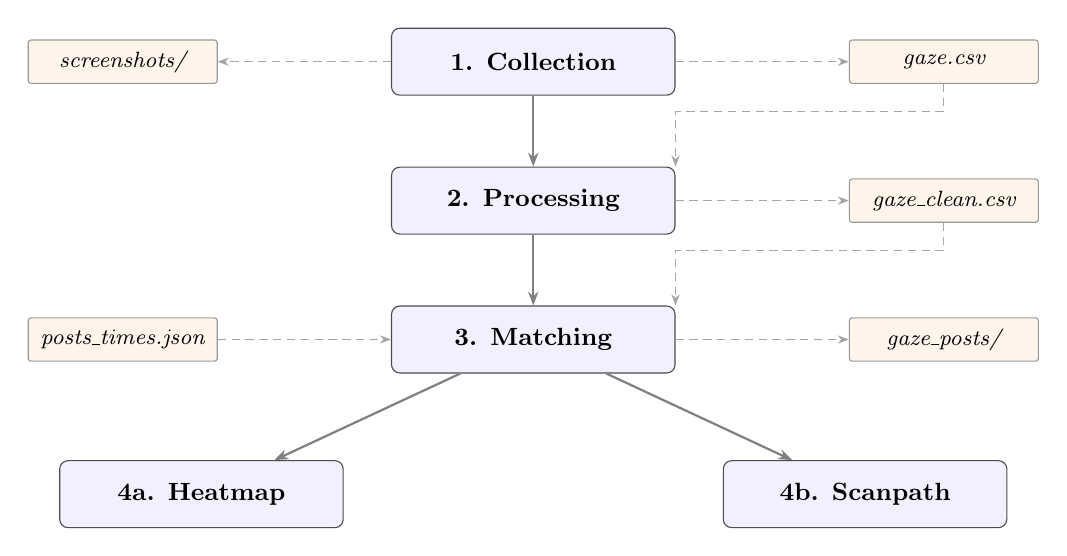
\begin{tikzpicture}[
      stage/.style={
        rectangle, rounded corners=3pt, draw=black!70, fill=blue!6,
        minimum width=3.6cm, minimum height=0.85cm, align=center,
        font=\small\bfseries},
      data/.style={
        rectangle, draw=black!40, fill=orange!8, rounded corners=1pt,
        minimum width=2.4cm, minimum height=0.55cm, align=center,
        font=\footnotesize\itshape},
      arr/.style={-{Stealth[length=5pt]}, thick, black!50},
      dataarr/.style={-{Stealth[length=4pt]}, black!35, densely dashed},
      node distance=0.9cm and 2.2cm
    ]
    % --- Stages (vertical spine) ---
    \node[stage] (collect) {1. Collection};
    \node[stage, below=of collect] (process) {2. Processing};
    \node[stage, below=of process] (match)   {3. Matching};
    \node[stage, below left=1.1cm and 0.6cm of match]  (heat) {4a. Heatmap};
    \node[stage, below right=1.1cm and 0.6cm of match] (scan) {4b. Scanpath};

    % --- Data artifacts ---
    \node[data, right=of collect] (raw)   {gaze.csv};
    \node[data, right=of process] (clean) {gaze\_clean.csv};
    \node[data, right=of match]   (posts) {gaze\_posts/};
    \node[data, left=of collect]  (shots) {screenshots/};
    \node[data, left=of match]    (json)  {posts\_times.json};

    % --- Stage arrows ---
    \draw[arr] (collect) -- (process);
    \draw[arr] (process) -- (match);
    \draw[arr] (match)   -- (heat);
    \draw[arr] (match)   -- (scan);

    % --- Data arrows ---
    \draw[dataarr] (collect) -- (raw);
    \draw[dataarr] (collect) -- (shots);
    \draw[dataarr] (raw.south)   -- ++(0,-0.35) -| (process.north east);
    \draw[dataarr] (process) -- (clean);
    \draw[dataarr] (clean.south) -- ++(0,-0.35) -| (match.north east);
    \draw[dataarr] (json)  -- (match);
    \draw[dataarr] (match) -- (posts);
  \end{tikzpicture}
  \caption{Pipeline architecture. Solid arrows show stage sequence;
    dashed arrows show data flow.}
  \label{fig:architecture}
\end{figure}

The system requires a Tobii Pro eye tracker, the Tobii Pro Eye Tracker
Manager for calibration, and a backend server on \texttt{localhost:3001}
providing post metadata.

% =============================================================================
\section{Data Collection}
\label{sec:collection}

Gaze data is collected via the Tobii Pro SDK using an asynchronous
callback. Each sample provides normalized display coordinates
$(l_x, l_y, r_x, r_y) \in [0,1]$ for both eyes, with microsecond SDK
timestamps and ISO\,8601 wall-clock times. Concurrently, screenshots are
captured via PyAutoGUI with timestamped filenames that later serve as
metadata for the matching stage.

% =============================================================================
\section{Gaze Data Processing}
\label{sec:processing}

\paragraph{Binocular averaging.}
Left and right eye coordinates are averaged into a single gaze point:
$\bar{x} = (l_x + r_x)/2$. When one eye is missing, the system falls
back to the available eye.

\paragraph{Coordinate normalization.}
Normalized $[0,1]$ coordinates are mapped to pixel space by multiplying
by display dimensions ($1920 \times 1080$ by default).

\paragraph{Gap interpolation.}
Contiguous NaN sequences are filled via linear interpolation between
the last valid and next valid samples, preserving smooth trajectories
during brief tracking losses.

% =============================================================================
\section{Gaze-to-Post Matching}
\label{sec:matching}

A backend server provides JSON metadata per post, including start/end
times relative to the recording origin. Each gaze sample is assigned to
the post whose time window contains its timestamp; samples outside all
windows are discarded. Screenshots are matched using the same temporal
criterion via their filename timestamps.

% =============================================================================
\section{Visualization}
\label{sec:visualization}

\subsection{Gaussian Heatmaps}

Gaze density is estimated by accumulating a 2D Gaussian kernel
($200 \times 200$\,px, $\sigma = g/6 \approx 33$\,px) at each gaze
point. Kernels at display edges are clipped rather than discarded.
Values below the non-zero mean are masked, and the result is rendered
with the \emph{jet} colormap at $\alpha = 0.5$ over the post screenshot
(Figure~\ref{fig:visualizations}a).

\subsection{Scanpath Plots}

Fixations are detected with a dispersion-based method: consecutive
gaze points within a 450\,px radius are grouped into a single fixation.
When the distance exceeds this threshold, a new fixation begins.
Fixation circles are sized proportionally to $\log(d_f)/\log(d_{\max})$,
connected by saccade lines, and labeled with sequential indices
(Figure~\ref{fig:visualizations}b).

\begin{figure}[ht]
  \centering
  \begin{subfigure}[t]{0.48\linewidth}
    \centering
    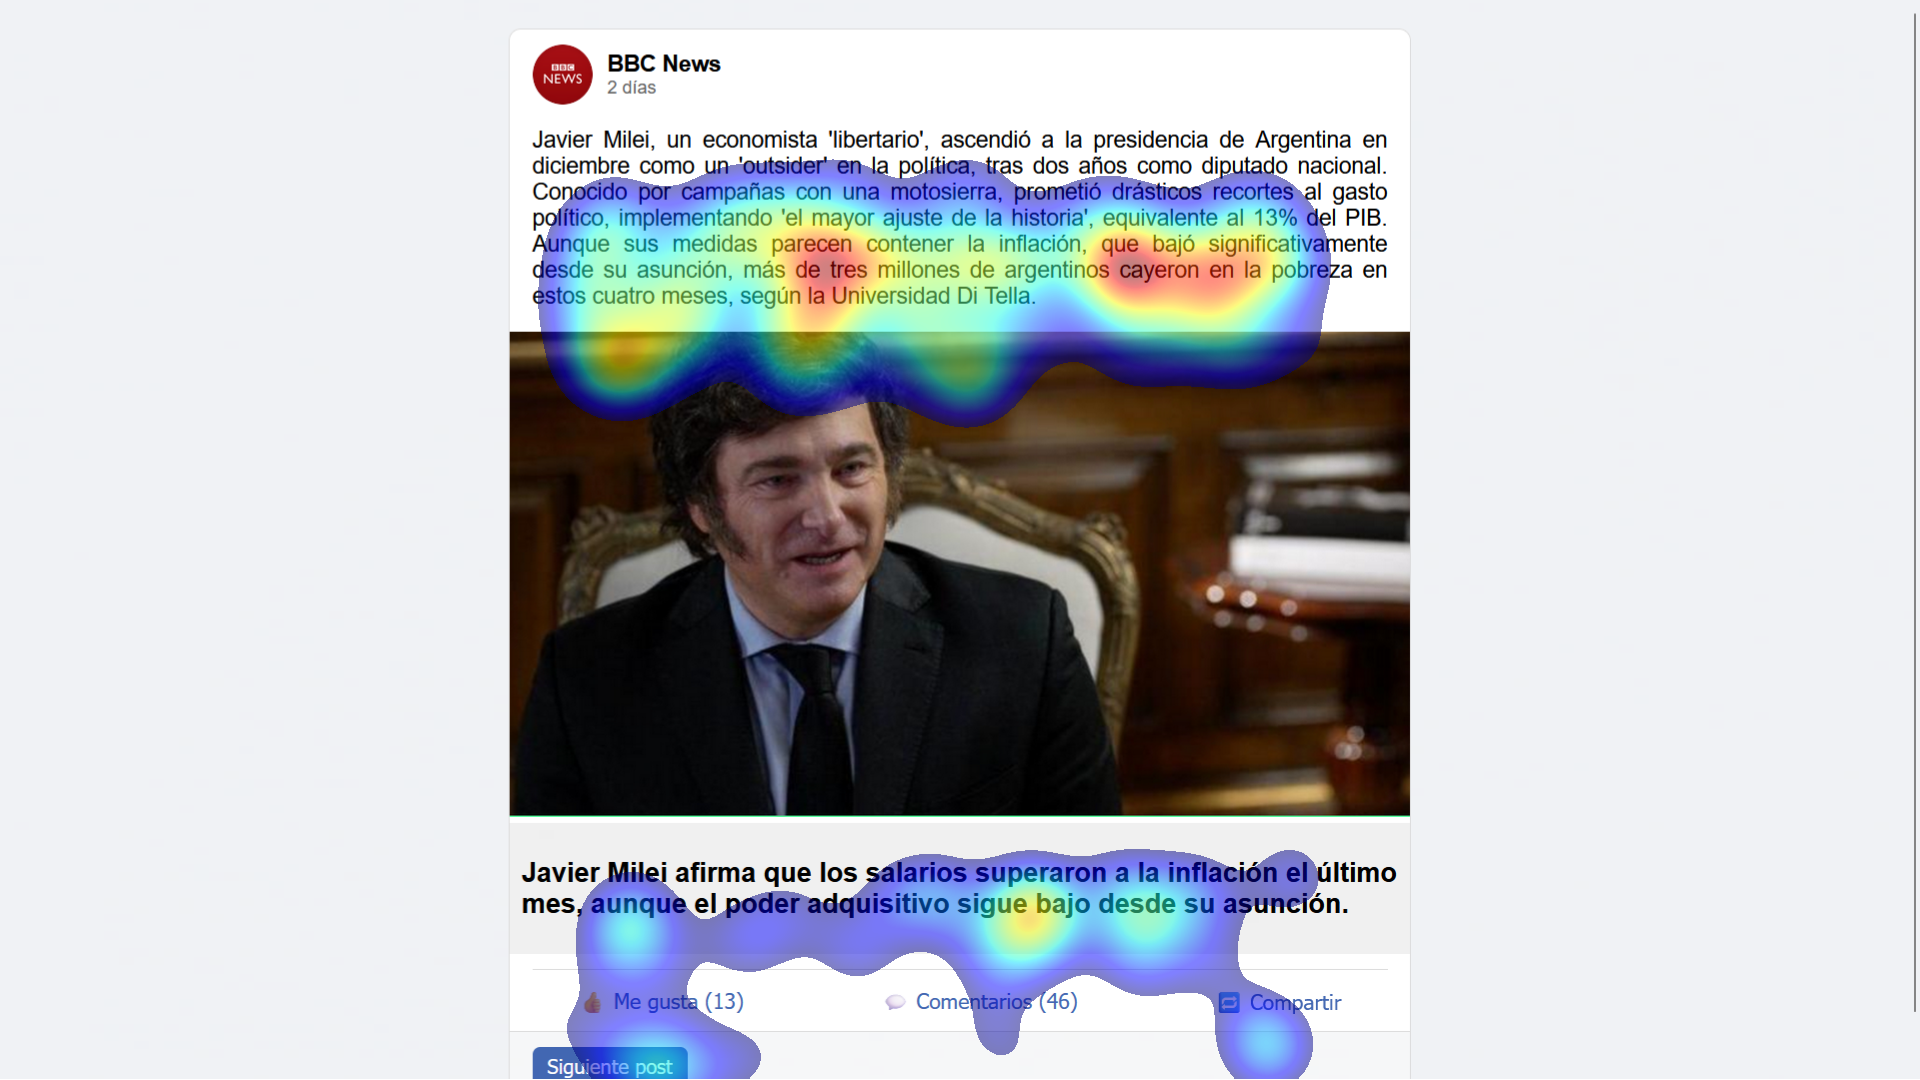
\includegraphics[width=\linewidth]{figures/heatmap_example.png}
    \caption{Gaussian heatmap}
    \label{fig:heatmap}
  \end{subfigure}
  \hfill
  \begin{subfigure}[t]{0.48\linewidth}
    \centering
    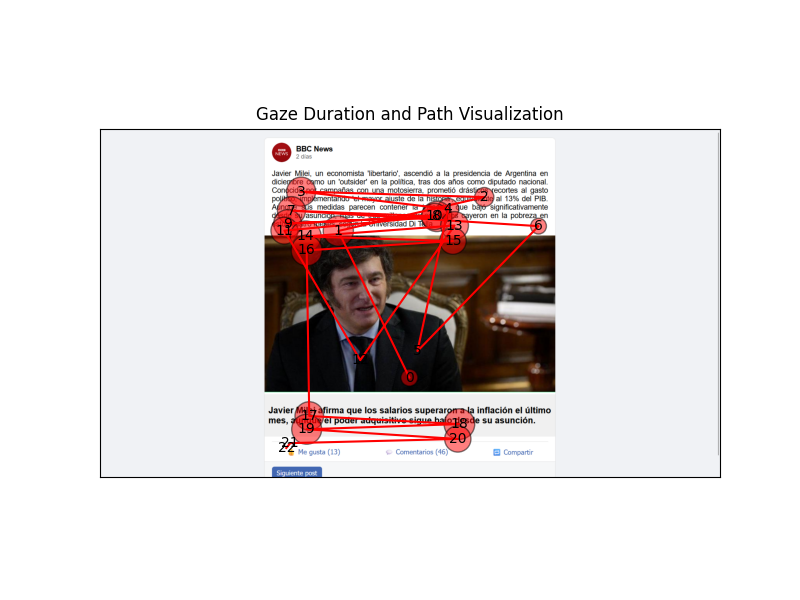
\includegraphics[width=\linewidth]{figures/scanpath_example.png}
    \caption{Scanpath plot}
    \label{fig:scanpath}
  \end{subfigure}
  \caption{Example visualizations for a single post.
    (a)~Heatmap: warm colors indicate high fixation density.
    (b)~Scanpath: circle size $\propto$ log-duration; numbers show
    viewing order.}
  \label{fig:visualizations}
\end{figure}

% =============================================================================
\section{Pipeline Parameters}
\label{sec:parameters}

Table~\ref{tab:params} summarizes default parameters. All are
configurable via command-line arguments.

\begin{table}[ht]
  \centering
  \caption{Default pipeline parameters.}
  \label{tab:params}
  \begin{tabular}{@{}llrl@{}}
    \toprule
    \textbf{Stage} & \textbf{Parameter} & \textbf{Default} & \textbf{Description} \\
    \midrule
    Collection & Sampling rate       & $\sim$60\,Hz       & Device-dependent \\
    Collection & Display size        & 1920$\times$1080   & Pixels \\
    Processing & Interpolation       & Linear             & Gap filling \\
    Heatmap    & Kernel size         & 200\,px            & Gaussian width \\
    Heatmap    & $\sigma$            & $\approx$33\,px    & Kernel spread \\
    Heatmap    & Transparency        & 0.5                & Overlay alpha \\
    Scanpath   & Fixation radius     & 450\,px            & Dispersion threshold \\
    Scanpath   & Circle scaling      & Logarithmic        & Duration mapping \\
    \bottomrule
  \end{tabular}
\end{table}

% =============================================================================
\section{Implementation}
\label{sec:implementation}

The pipeline runs on Python~3.10+ with Matplotlib, NumPy, Pandas,
PyAutoGUI, and the Tobii Research SDK. Dependencies are managed with
\texttt{uv}~\citep{uv2024}; code quality with Ruff, ty, and Bandit.
A batch utility processes multiple participants in parallel.

% =============================================================================
\section{Future Work}
\label{sec:future}

Planned extensions include: velocity-based fixation detection
(I-VT)~\citep{salvucci2000identifying}, automatic AOI extraction via
computer vision, advanced smoothing (Savitzky--Golay), real-time
visualization during recording, and cross-platform support.

% =============================================================================
\section{Conclusion}
\label{sec:conclusion}

FacebookEyeTracker provides a modular, open-source solution for
eye-tracking studies on social media. Its automatic gaze-to-post matching
and dual visualization outputs make it a practical tool for HCI
researchers. Code available at
\url{https://github.com/sebastianbreguel/FacebookEyeTracker}.

% =============================================================================
\bibliographystyle{plainnat}
\bibliography{references}

\end{document}
